%        File: ans_2013_therm.tex
%     Created: Mon Aug 13 10:00 AM 2012 C
%

%% To use the glossaries acronym package, you'll need to define any acronyms you intend to 
%% use. You can define acronyms with \newacronym{label}[acronym]{written out form}
%% To refer to them in the text use \gls{label}

\documentclass{anstrans}
%%%%%%%%%%%%%%%%%%%%%%%%%%%%%%%%%%%
\usepackage[acronym,toc]{glossaries}
\include{acros}
\makeglossaries

% concise yet adequately descriptive title
\title{Dynamic Determination of Thermal Repository Capacity For Fuel Cycle Analysis}
\author{Kathryn D.~Huff$^1$, Alexander T. Bara$^2$}

%% uncomment these next five only if using anstrans
\institute{$^1$Univ. of Wisconsin, 1500 Engineering Dr., Madison, WI, 53706\\ 
\& Argonne National Laboratory, 9700 S. Cass Ave., Lemont, IL, katyhuff@gmail.com\\
$^2$Univ. of Illinois, Urbana Champaign, IL, 61801, bara1@illinois.edu}
\usepackage{graphicx}
\usepackage{booktabs} % nice rules for tables
\usepackage{microtype} % if using PDF
\newcommand{\units}[1] {\:\text{#1}}%
\newcommand{\SN}{S$_N$}%{S$_\text{N}$}%{$S_N$}%

\date{}
%%%%%%%%%%%%%%%%%%%%%%%%%%%%%%%%%%%
\begin{document}
%%%%%%%%%%%%%%%%%%%%%%%%%%%%%%%%%%%%%%%%%%%%%%%%%%%%%%%%%%%%%%%%%%%%%%%%%%%%%%%%
\section{Introduction}
% Provide a summary of the work conducted:
%      Describe the technical problem clearly
%      support it with a method

An algorithm and supporting database for rapid thermal repository capacity 
calculation implemented in Cyder, a software library for coupled thermal and 
hydrologic repository performance analysis, is described. Integration of Cyder 
with the Cyclus fuel cycle simulator is also described. Finally, a proof of 
principle demonstration is presented in which the rapid calculation method 
described here is compared with results of a more detailed model.

This algorithm employs a \gls{STC} method 
\cite{radel_effect_2007, radel_repository_2007} and has 
resulted from combining detailed spent nuclear fuel composition data 
\cite{carter_fuel_2011} with a
detailed thermal repository performance analysis tool from 
\gls{LLNL} and the \gls{UFD} campaign \cite{greenberg_application_2012}. By 
abstraction of and benchmarking against these detailed thermal models, Cyder 
captures the dominant 
physics of thermal phenomena affecting repository capacity in various geologic 
media and as a function of spent fuel composition.

Abstraction based on detailed computational thermal repository performance 
calculations has resulted in implementation of the \gls{STC} estimation 
algorithm and a supporting reference dataset.  This method is capable of 
rapid estimation of temperature increase near emplacement tunnels as a function 
of waste composition, limiting radius, $r_{lim}$, waste package spacing, $S$, 
near 
field thermal conductivity, $K_{th}$, and near field thermal diffusivity, 
$\alpha_{th}$.

\section{Motivation}
% Provide a brief description of the importance of the work (what problem it 
%   addresses/solves):

The United States is simultaneously considering a number of domestic nuclear 
fuel cycle and geologic disposal options \cite{doe_strategy_2013}.  These decisions are technologically 
coupled by repository capacity. That is, the thermal capacity of a geologic 
repository is a strong function of site geology thermal parameters (see Table 
\ref{tab:heat_tab}) as well as spent fuel composition, which varies among 
alternative fuel cycles. 

To inform research and development in this coupled system, a generic geologic disposal 
performance model capable of dynamic integration with a systems analysis 
framework is necessary to illuminate capacity constraints and dynamic feedback 
effects of candidate repository geologies in the context of fuel cycle options.
In answer to this need, the algorithm in this work has been implemented in the 
Cyder software library which integrates with the Cyclus computational 
fuel cycle systems analysis platform \cite{huff_cyder_2013,wilson_cyclus:_2012}. 

%        File: heat_tab.tex
%     Created: Thu Aug 04 11:00 AM 2011 C
% Last Change: Thu Aug 04 11:00 AM 2011 C
%
\begin{table}[h!]
  \centering
  \footnotesize{
  \begin{tabular}{|l|r|r|r|r|}
    \multicolumn{5}{c}{\textbf{Thermal Behavior of Various Concepts}}\\
    \hline
    Feature & Clay & Granite & Salt & Deep Borehole \\ 
            & (Bentonite & (Concrete & (Salt & (Bentonite\\ 
            & Buffer) & Buffer) & Backfill) & Buffer) \\ 
    \hline
    Buffer Limit $[^{\circ}C]$ & 100  & 100  & 180 & 100  \\ 
    Reference
    & \cite{hardin_generic_2011}   
    & \cite{von_lensa_red-impact_2008}   
    & \cite{von_lensa_red-impact_2008,brewitz_long-term_2002,carter_thermal_2011}   
    & \cite{von_lensa_red-impact_2008}  \\ 
    &      &      &     &      \\
    Host Limit $[^{\circ}C]$   & 100  & 200  & 180 & none \\ 
    Reference                     
    & \cite{<++>}   
    & \cite{<++>}   
    & \cite{<++>}   
    & \cite{<++>}   \\
    &      &      &     &      \\
    $\alpha_{th} [\frac{10^{-6}m^2}{s}]$ & $0.12-0.19$ & $0.9-1.8$ & $1.3-2.1$ & $0.9-1.8$ \\ 
    Reference                     
    & \cite{tikhonravova_effect_2007} 
    & \cite{durham_thermal_1987,hardin_generic_2011,kim_thermal_2007}     
    & \cite{hardin_generic_2011,nieland_storage_2001}   
    & \cite{durham_thermal_1987,hardin_generic_2011,kim_thermal_2007}   \\ 
    &      &      &     &      \\
    $K_{th} [\frac{W}{m{\cdot}K}]$ & $1-2$ & $2-4$ & $\sim4$  & $2-4$ \\ 
    Reference                     
    & \cite{hardin_generic_2011,tikhonravova_effect_2007}    
    & \cite{hardin_generic_2011,kim_thermal_2007,surma_porosity_2003,ab_long-term_2006}    
    & \cite{hardin_generic_2011,nieland_storage_2001}
    & \cite{hardin_generic_2011,kim_thermal_2007,surma_porosity_2003}\\ 
    &      &      &     &      \\
    Coalesence & yes & no & yes & no \\ 
    \hline
  \end{tabular}
  \caption[Models for Heat Transport for Various Geologies]{Maximum heat load constraints, thermal 
  diffusivities, and thermal conductivities vary among repository concepts and host formations. }
  }
  \label{tab:heat_tab}
\end{table}


A generic repository model appropriate for systems analysis must emphasize 
modularity and speed while providing modeling options at various levels of 
detail. Therefore, parameterized simulations and abstraction efforts conducted to develop 
the method described in this work sought to capture the dominant physics of 
thermal repository capacity assessment so that the Cyder disposal environment 
library could meet the simulation speed requirements of the Cyclus fuel cycle 
simulator.



\section{Methodology}
% How did you get such fabulous results?
%       in reproducible detail

% Incorporation in cyclus (discuss capacity estimation, briefly.)
\subsubsection{Cyder Integration With Cyclus}

To inform dynamic behavior within the simulator, the repository requires 
a model capable of quickly arriving at a heat based 
capacity for an arbitrary waste stream. 

More specifically, the Cyder repository model is a type of FacilityModel 
(see \cite{wilson_cyclus:_2012}) within 
Cyclus and interfaces with the simulation by requesting materials from the fuel 
cycle facilities operating simultaneously with it. It the receives materials 
according to the capacity that it defines. In the case of Cyder, the 
heat-limited capacity of the repository is reassessed for each new waste 
stream composition offered to the repository.




% Specific Temperature Change


\subsubsection{Specific Temperature Change Method}
Introduced by Radel, Wilson et. al., the Specific Temperature Change method uses 
a linear approximation to arrive at the thermal loading density limit.  
When the thermal time constant of the rock is much shorter than the waste form 
decay package, the change in package wall temperature can be described by 

\begin{align}
\Delta T_1 &= q(t_0)\rho_{limit}C'
\intertext{where}
\Delta T_1 &= T_{lim} - T_{amb} \nonumber\\
T_{lim} &= \mbox{ Temperature limit }[^{\circ}C]\nonumber\\
T_{amb} &= \mbox{ Ambient rock temperature }[^{\circ}C]\nonumber\\
q(t_0) &= \mbox{ Heat at the inital time} \nonumber \\
\rho_{limit} &= \frac{C_1}{Q_1}\nonumber\\
C' &= \mbox{ Thermal constant }[-]\nonumber\\
\Delta T &= T_{lim}-T_{amb}[^{\circ}C]\nonumber\\
\end{align}

Figure \ref{fig:CmScaling} demonstrates the scaling of an STC curve to represent 
the heat from $25.9g$ of initial $^{242}Cm$. 

\begin{figure}[htp!]
\begin{center}
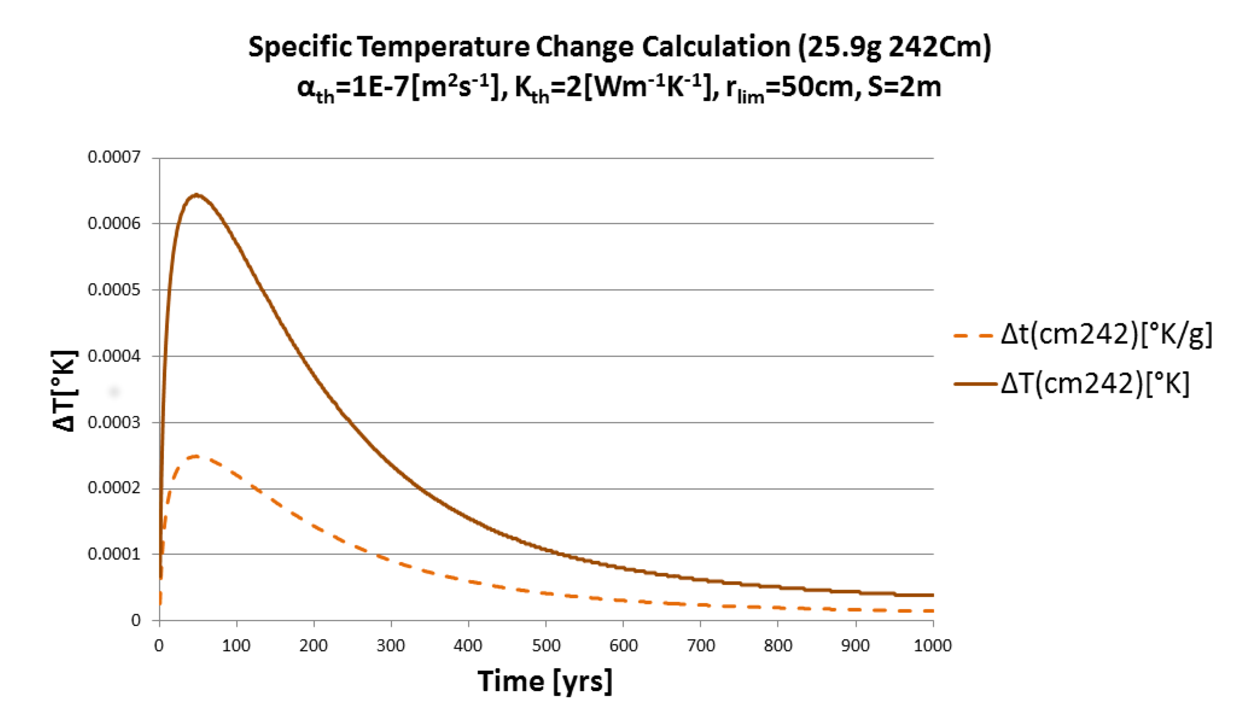
\includegraphics[width=\columnwidth]{images/CmScaling.eps}
\end{center}
\caption{As a demonstration of the calculation procedure, the temperature change 
  curve for one intial gram of $^{242}Cm$ and is scaled to represent $25.9g$, 
  approximately the $^{242}Cm$ inventory per MTHM in 51GWd burnum UOX PWR fuel. }
\label{fig:CmScaling}
\end{figure}

For an arbitrary waste stream 
composition, scaled curves calculated in this manner can be superimposed for 
each heat generating isotope to arrive at an approximate total temperature 
change at the calculation radius. 

To support this calculation in Cyder, a reference data set of temperature change 
curves, $\Delta t_i$, were calculated for high heat contributing isotopes. These 
curves were calclated as a function of specified repository spacing, $S$, heat 
limit radius, $r_{lim}$, and thermal paramters $\alpha_{th}$ and $K_{th}$. The 
total temperature change is the sum of the mass scaled curves,

\begin{align}
\Delta T &\sim \sum_{i\in H} m_i \Delta t_i(r,S,K_{th},\alpha_{th})
\intertext{where}
\Delta T &= \mbox{ total temperature change in waste }[^{\circ}K]\nonumber\\
H &= \mbox{ set of high heat isotopes }[-]\nonumber\\
m_i &= \mbox{ mass of isotope i  } [g]\nonumber\\
\Delta t_i(r,S,K_{th},\alpha_{th}) &= \mbox{ temperature change due to 1 g of i }[^{\circ}K].\nonumber
\label{superposition}
\end{align}

The use of this superposition is demonstrated in Figure 
\ref{fig:CmSuperposition}.

\begin{figure}[ht!]
\begin{center}
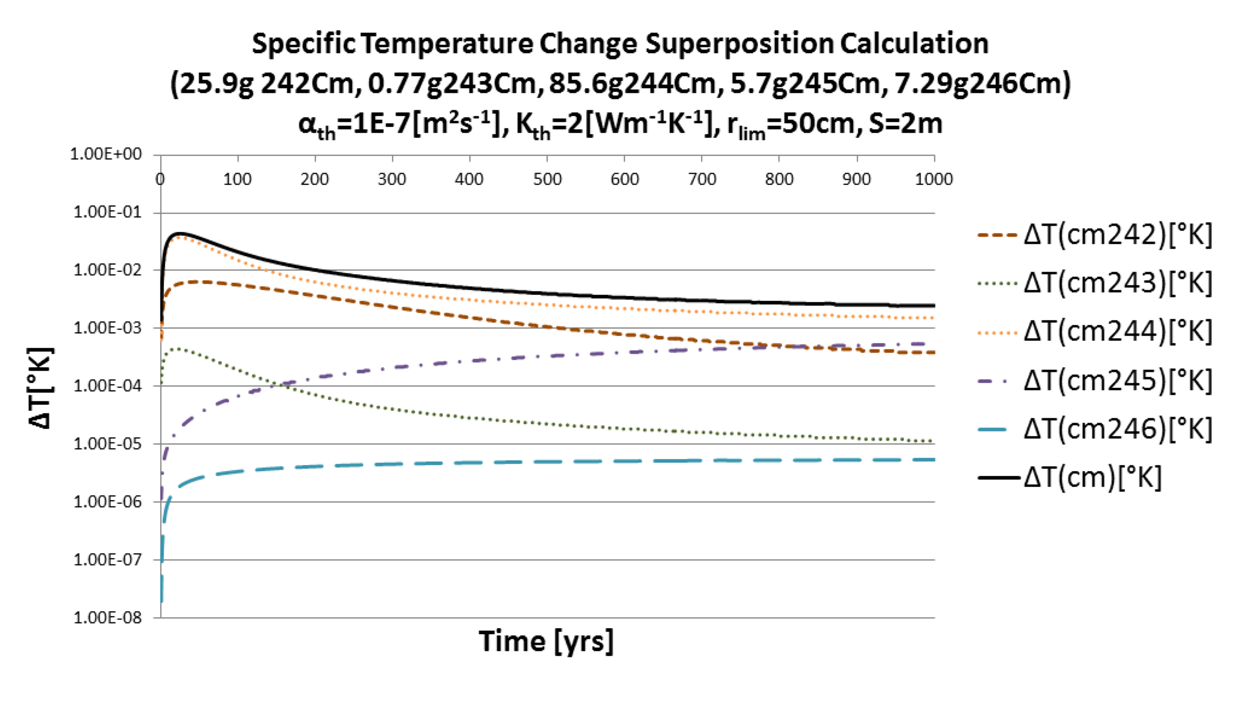
\includegraphics[width=\columnwidth]{images/CmSuperposition.eps}
\end{center}
\caption{As a demonstration of the calculation procedure, scaled temperature change 
  curves for two isotopes are superimposed to achieve a total temperature 
change (note log scale).}
\label{fig:CmSuperposition}
\end{figure}



% LLNL Mathcad Model (range table)
% LLNL

\begin{frame}[ctb!]
\frametitle{LLNL Model : Background}
The analytical  model
\begin{itemize} 
  \item was created at LLNL (H. Greenberg, J. Blink, et. al) \cite{hardin_generic_2011, sutton_investigations_2011, 
greenberg_application_2012}
  \item employs an analytic model from Carslaw and Jaeger \cite{carslaw_conduction_1959} 
  \item is implemented in MathCAD \cite{ptc_mathcad_2010}
  \item seeks to inform heat limited waste capacity calculations for 
    \begin{itemize}
      \item arbitrary geology 
      \item arbitrary waste package loading densities
      \item arbitrary homogeneous decay heat source
    \end{itemize}
\end{itemize}
\end{frame}

\begin{frame}
  \frametitle{LLNL Model : Geometry}
  \begin{figure}[h!]
    \begin{center}
      \includegraphics[width=0.7\columnwidth]{images/llnlConcept.eps}
    \end{center}
    \caption{Vertical, horizontal, alcove, and borehole emplacement layouts can 
    be represented by a line of point sources and adjacent line sources 
    \cite{sutton_investigations_2011}.}
    \label{fig:llnl}
  \end{figure}
\end{frame}



% Supporting data from Joe Carter (heat per iso)

% Interpolation (figure this out, or be vague?)

\section{Results and Analysis}
% Provide your results:
%       clearly

The primary outcome of this work is a mulitdimensional database of repository temperature 
change per mass of high heat contributing isotopes supporting the implementation 
of the Specific Temperature Change Method in Cyder. 

A validation effort concerning this tool was performed to assess the validity of 
the Specific Temperature Change method for the purpose of repository thermal 
response estimation. 



THE RESULT IS BOUNDED.

% Unit Test Results
For verification of code In addition to the suite of unit tests performed on these analytics which test 
the behavior of the interpolation and specific temperature change algorithms.

% Benchmarking Efforts

Comparing the results of this method with the \gls{LLNL} model gave 
appropriately similar results. 


% Base Case Demonstration ???
The base case demonstration of integration with the Cyclus next generation 
fuel cycle simulator.


\section{Conclusions}
% Was: Importance to Others - Replace with a conclusion.
The Cyder source code in which these models are implemented as well as 
associated documentation are freely available for use by model developers in the 
field of nuclear waste management. The application programming interface to this 
software library is intentionally general to facilitate the incorporation of the 
models presented here within software tools in need of a multicomponent repository 
model.

Furthermore, this work contributes to an expanding ecosystem of computational 
models available for use with the Cyclus fuel cycle simulator. The Cyder thermal 
response and hydrologic 
nuclide transport library, by virtue of its capability to modularly integrate 
with the Cyclus fuel cycle simulator, has laid the foundation for integrated 
disposal option analysis in the context of fuel cycle options. 

\input{acks}

%%%%%%%%%%%%%%%%%%%%%%%%%%%%%%%%%%%%%%%%%%%%%%%%%%%%%%%%%%%%%%%%%%%%%%%%%%%%%%%%
%\nocite{*}
\bibliographystyle{ans}
\bibliography{ans_2013_therm}
\end{document}



